\subsection{Kodierung}

Die Kodierung wurde identisch wie in der Masterarbeit \citep{Sichau2015a} durchgeführt.

\subsection{Unterschiede zwischen den Tests}

Die Unterschiede der Testergebnisse auf Ebene der Qualitätsstandards und der erreichten Qualitätslevel wurden bereits in der Masterarbeit untersucht. In dieser Arbeit soll der Fokus deshalb auf die Item-Ebene gelegt werden.

\begin{table}[htbp]
  \centering
\begin{tabular}{@{}lllllllll@{}}
\toprule   &  \multicolumn{2}{c}{201 vs 305} &&  \multicolumn{2}{c}{301 vs 305}  && \multicolumn{2}{c}{201 vs 301}\\
 \cmidrule{2-3}  \cmidrule{5-6} \cmidrule{8-9}
Item  & $p$ & $\rho$ &&  $p$ & $\rho$ &&  $p$ & $\rho$\\
\midrule
 1.1 & 0.13 & 0.18  && 0.54 & -0.07 && 1e-3 & 0.36 \\ 
 1.2 & 0.02 & 0.26  && 0.19 & -0.16 && 0.27 & 0.13 \\ 
 2.1 & 2e-6 & 0.52  && 0.07 & 0.21  && 6e-3 & 0.32\\ 
 3.1 & 0.88 & 0.02  && 0.89 & 0.01  && 0.33 & -0.12\\ 
 3.2 & 0.13 & 0.18  && 0.15 & 0.17  && 1e-3 & 0.36\\ 
 4.1 & 0.04 & 0.24 && 0.12 & 0.18  	&& 0.07 & 0.21 \\ 
 4.2 & 0.13 & 0.18 && 1 & 0  		&& 0.18 & 0.15 \\ 
 4.3 & 0.73 & -0.04  && 0.81 & -0.02  && 0.73 & -0.04 \\ 
 4.4 & 0.73 & -0.04  && 0.81 & -0.02  && 0.73 & -0.04 \\ 
 5.1 & na. & na.  && 0.89 & 0.02  	&& na. & na. \\ 
 5.2 & 2e-4 & 0.41  && 8e-4 & 0.38  && 2e-4 & 0.42 \\ 
\bottomrule

\end{tabular} 
  \caption{Spearmans-$\rho$ und der p-Wert für Korrelationstest auf Item-Ebene. Für die drei Tests 201 (Chemie Temperatur), 301 (Physik Kraft) und 305 (Physik Temperatur)}
  \label{tab:cor}
\end{table}

Daher wurden Korrelationstest zwischen den einzelnen Tests auf Item-Ebene durchgeführt. Da keine Annahme über die Verteilung der Items gemacht wurde, wurde der Speramans Rangkorrelationskoeffizient berechnet. Bei einigen Items war dies nicht möglich, da alle Schülerinnen und Schüler dort keine Antworten gegeben haben. Die Ergebnisse dieses Testes befinden sich in Tabelle \ref{tab:cor}.

\subsection{Rasch Analyse}

Zusätzlich wurden die Items noch mit Hilfe dem partial-credit Modell analysiert. Das partial-credit Modell wurde gewählt, da die Items nicht dichotom verteilt sind. Sondern teilweise auch Werte zwischen 0 und 2 annehmen können.

Auf-Item Ebene konnte das Rasch-Modell nicht mit Hilfe des Andersens Likelihood-
Quotienten Test validiert werden. Auch durch Ausschluss von Items wurde der p-Wert nicht verbessert. Das besste Modell mit einem p-Wert von 0.016 konnte für alle Items bis auf Item M201\_5.1 erreichte werden. Mit diesem Modell wurde die weitere Untersuchung durchgeführt.

Der Wald-Test, mit welche ungeeignete Items identifiziert werden können, führte zu folgenden "`schlechten"' Items: M201\_1.1, M201\_3.1, M305\_4.1, M305\_5.2.
Die Items M201\_4.2 M201\_4.3 M201\_4.4 M201\_5.2 M301\_4.3 M301\_4.4 M305\_4.2 M305\_4.3 M305\_4.4 M201\_2.1 M305\_2.1 und M301\_5.1 wurden aufgrund zu geringer Datenqualität bereits ausgeschlossen. Die Ergebnisse des Testes sind in Darstellung \ref{fig:GOF} grafisch dargestellt.

\begin{figure}[htp]
   \centering
   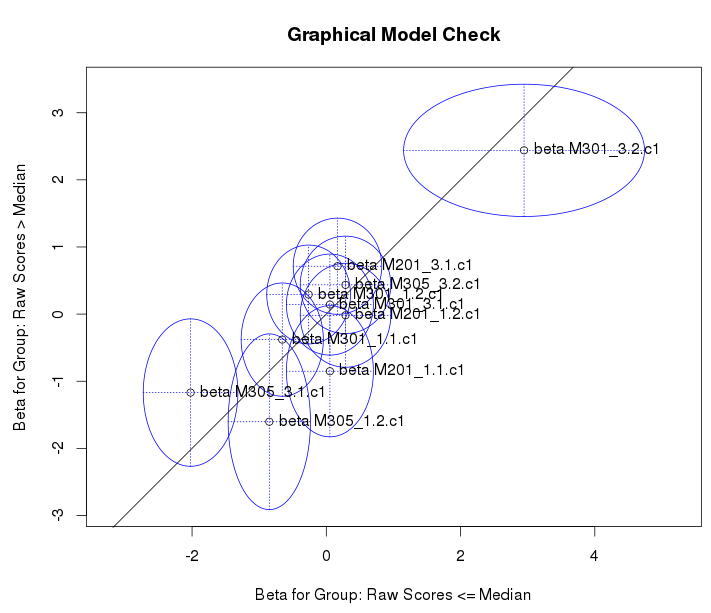
\includegraphics[width=1.0\linewidth]{graphics/GOF.png}
   \caption{Modellkontrolle des Rasch-Modells: mehrere Items haben eine
   signifikante Abweichung von der Diagonalen, daher gibt es bei diesen einen si-
   gnifikanten Unterschiede für Personen mit niedrigen und hohen Rand-
   summen in den Items.}
   \label{fig:GOF}
\end{figure}


Nachdem das Modell versucht wurde zu validieren wurde trotzdem noch untersucht, inwiefern die Items einen unterschiedlichen Schwierigkeitsgrad aufweisen. Die Resultate dieser Analyse sind in Darstellung \ref{fig:PIM} dargestellt.



\begin{figure}[htp]
   \centering
   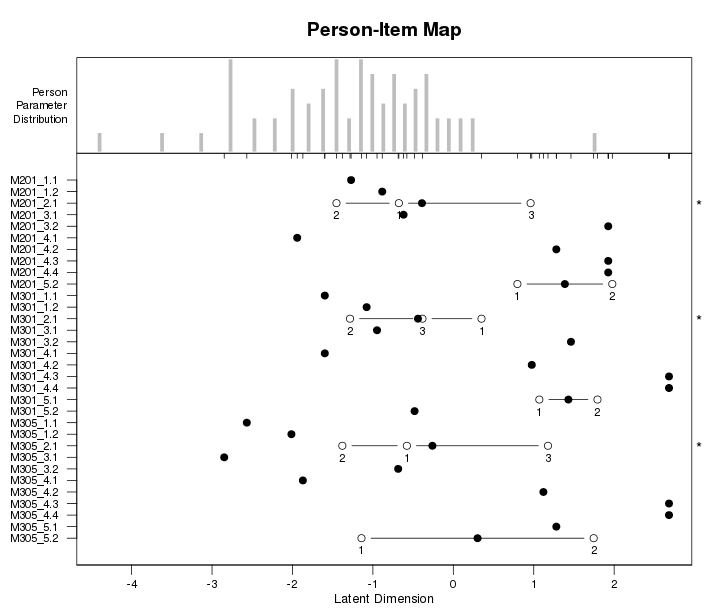
\includegraphics[width=1.0\linewidth]{graphics/PersonItemMap.png}
   \caption{Person-Item-Map des partial-credit Modells der einzelnen Items.}
   \label{fig:PIM}
\end{figure}

